\documentclass{beamer}
\setbeamercovered{transparent}

\usepackage{epstopdf}
\usepackage[inline]{asymptote}

\mode<presentation> %?

\usetheme{Frankfurt}
\usepackage{helvet}
\usepackage{mathptmx}
%\usefonttheme{professionalfonts}
\usefonttheme[onlymath]{serif}
\usefonttheme{structurebold}

%\renewcommand{\familydefault}{Futura}
%\setsansfont{Verdana}

\setlength{\unitlength}{\paperwidth}

% width, height, title, content
\newcommand{\SizedBlock}[4]{
  \begin{block}{#3}
    \parbox[t][#2\paperwidth][t]{#1\paperwidth}{#4}    
  \end{block}
}

% w1, c1, w2, c2
\newcommand{\TwoColumns}[4]{
  \vspace{-0.02\paperwidth}
  \begin{columns}[t]
    \begin{column}{#1\paperwidth}
      #2
    \end{column}\hspace{-0.02\paperwidth}
    \begin{column}{#3\paperwidth}
      #4
    \end{column}
  \end{columns}
}

% w1, c1, w2, c2, w3, c3
\newcommand{\ThreeColumns}[6]{
  \vspace{-0.02\paperwidth}
  \begin{columns}[t]
    \begin{column}{#1\paperwidth}
      #2
    \end{column}\hspace{-0.07\paperwidth}
    \begin{column}{#3\paperwidth}
      #4
    \end{column}\hspace{-0.07\paperwidth}
	\begin{column}{#5\paperwidth}
      #6
    \end{column}
  \end{columns}
}

% height, title1, content1, title2, content2
\newcommand{\TwoColumnBlocksW}[6]{
  \TwoColumns{
        #6}{
        \SizedBlock{#6}{#1}{#2}{#3}}{
        #6}{
        \SizedBlock{#6}{#1}{#4}{#5}}
}

% height, title1, content1, title2, content2
\newcommand{\TwoColumnBlocks}[5]{
  \TwoColumnBlocksW{#1}{#2}{#3}{#4}{#5}{0.4}
}

% height, title1, content1, title2, content2, title3, content3
\newcommand{\ThreeColumnBlocks}[7]{
  \ThreeColumns{
        0.24}{
        \SizedBlock{0.24}{#1}{#2}{#3}}{
        0.24}{
        \SizedBlock{0.24}{#1}{#4}{#5}}{
        0.24}{
        \SizedBlock{0.24}{#1}{#6}{#7}}
}

\newcommand{\PutPic}[3]{
  \put(#1){\includegraphics[#2\paperwidth]{./img/#3}}
}

\usepackage{color}
\usepackage{fancybox}

\begin{document}
\title{Particle-Based Anisotropic\\ Surface Meshing\\
\small{Zichun Zhong et.al Sig 2013}}
\author{Tengfei Jiang}

\newcommand{\FPP}[2]{\frac{\partial #1}{\partial #2}}
\begin{frame}
  \titlepage
\end{frame}

\begin{frame}{Pipeline}
  \begin{enumerate}
    \item Motivation 
    \item Background
    \item Key Idea
    \item Algorithm
    \item Results
    \item Conclusion
  \end{enumerate}
\end{frame}

\section{Motivation}
\begin{frame}{Prolog}
\begin{figure}
\centering
\includegraphics[height=1.4in]{./img/introduction.png}
\end{figure}
\end{frame}

\begin{frame}{Motivation}
\begin{itemize}
\item 
To satisfy user shape size requirement.
\begin{figure}
\includegraphics[height=1.5in]{./img/size.png}
\end{figure}
\item Related to optimal approximation of a function with piecewise-linear elements
\end{itemize}
\end{frame}


\section{Related Work}
\begin{frame}{Background}
\begin{itemize}
\item Metric
\item Anistropoy
  \begin{block}{}
    \[<v,w>_{M(x)}=v^TM(x)w\]
    \ovalbox{$M(x)$} is the metric defined at $x$.
  \end{block}
\end{itemize}
\end{frame}

\section{Key Idea}
\begin{frame}{Key Idea}
\begin{block}{Key}
Optimize an uniform isotropic distribution of particles in higher dimension space to get anistropic one in low dimension space.
\end{block}
\begin{figure}[!htb]
\includegraphics[height=2.0in]{./img/space.png}
\end{figure}
\end{frame}

\section{Algorithm}
\begin{frame}{Algorithm}
\begin{figure}[!htb]
\includegraphics[height=2.0in]{./img/overview.png}
\end{figure}
\end{frame}

\begin{frame}{Optimize particle location}
\begin{block}{}
[Witkin And Heckbert 1994] Minimizing pair-wise Gaussian energy leads to a uniform isotropic distribution of particles
\end{block}
\begin{eqnarray*}
E^{ij} &=&e^{-\frac{\|x_i-x_j\|^2}{4\sigma^2}}\\
F^{ij} &=& \frac{\partial E^{ij}}{\partial x_j} = \frac{(x_i-x_j)}{2\sigma^2}e^{-\frac{\|x_i-x_j\|^2}{4\sigma^2}}
\end{eqnarray*}
Denote surface $\Omega$ is mapped to $\overline{\Omega}$ in a higher space. Thus the above equations are turned into:
\begin{eqnarray*}
\overline{E}^{ij} &=&e^{-\frac{\|\overline{x}_i-\overline{x}_j\|^2}{4\sigma^2}}\\
\overline{F}^{ij} &=& \frac{\partial \overline{E}^{ij}}{\partial \overline{x}_j} = \frac{(\overline{x}_i-\overline{x}_j)}{2\sigma^2}e^{-\frac{\|\overline{x}_i-\overline{x}_j\|^2}{4\sigma^2}}
\end{eqnarray*}
\end{frame}

\begin{frame}{Approximation}
To avoid really calculating mapping function, approximation based only on metric is involved.
\begin{itemize}
\item $\overline{v}=J(x)v$, $\overline{w}=J(x)w$, thus $<\overline{v},\overline{w}>=v^TJ(x)^TJ(x)w=v^TM(x)w$
\item $\overline{x_i}-\overline{x}_j\approx J_{ij}(x_i-x_j)$, $\|\overline{x}_i-\overline{x}_j\|^2=<\overline{x}_i-\overline{x}_j, \overline{x}_i-\overline{x}_j>\approx (x_i-x_j)^TM_{ij}(x_i-x_j)$  
\item $\overline{E}^{ij}\approx e^{-\frac{(x_i-x_j)^TM_{ij}(x_i-x_j)}{4\sigma^2}}$
\item $\overline{F}^{ij}\approx \frac{J_{ij}(x_i-x_j)}{2\sigma^2}e^{-\frac{(x_i-x_j)^T M_{ij}(x_i-x_j)}{4\sigma^2}}$ \ovalbox{$J_{ij}$} depends on mapping function, which needs to be approximate further.
\end{itemize}
\end{frame}

\begin{frame}{Approximate $J_{ij}$}
$M(x)$ can be decompositied(SVD) as $M(x)=R(x)^TS(x)^2R(x)$:
\begin{itemize}
\item Given $S(x),R(x)$: \quad $Q(x)=S(x)R(x)$, thus \doublebox{$M(x)=Q(x)^TQ(x)$}.
\item Given $M(x)$: \quad decomposition $M(x)=Q(x)^TQ(x)$ is not unique, but decomposition of $Q'(x)=\sqrt{M(x)}$ is. $Q'(x)=R(x)^TS(x)R(x)$, thus \doublebox{$M(x)=Q'(x)Q'(x)=Q'(x)^TQ'(x)$}.
\end{itemize}

Now, let's explore the relationship between $J_{ij}$ and $Q_{ij}$.
\end{frame}

\begin{frame}{$J_{ij}$ and $Q_{ij}$}
Using QR decomposition:
\[J_{ij} = U_{ij}\left [ \begin{array}{cc} P_{ij} \\ 0\end{array} \right ]\]
where $J_{ij}$ is a $\overline{m}\times m$ matrix. $\overline{m}$ is dimension of embedding space, and $m$ is 2 or 3 depends on $\Omega$ is a 2d domain or 3d domain. $U_{ij}$ is a unitary matrix.Then:
\[M_{ij}=J_{ij}^TJ_{ij}=P_{ij}^TP_{ij}\]

$P_{ij}=O_{ij}Q_{ij}$, where $O_{ij}$ is a rotation matrix. And $Q_{ij}$ stands for $Q_{ij},Q'_{ij}$ in last slide, since $Q'(x)=Q'(x)^T$.
\end{frame}

\begin{frame}{$J_{ij}$ and $Q_{ij}$}
\begin{eqnarray*}
J_{ij}&=&U_{ij}\left [ \begin{array}{cc} O_{ij}Q_{ij} \\ 0\end{array}  \right ]\\
&=&\underbrace{U_{ij}\left [ \begin{array}{cc} O_{ij} & 0 \\ 0 & I \end{array} \right ]}_{W_{ij}}\left [ \begin{array}{cc} Q_{ij} \\ 0\end{array}  \right ]
\end{eqnarray*}
Where $W_{ij}$ is a rotation matrix.

$W_{ij}$ can be approximated as $W_i$ if input metric is smooth. Thus:
\[J_{ij}v_{ij}\approx W_i \left [ \begin{array}{cc} Q_{ij}v_{ij} \\ 0\end{array}  \right ]\]
\end{frame}

\begin{frame}{Gradient $F$}
In $\overline{m}$ dimension, force is:
\begin{eqnarray*}
\overline{F}^{ij}&=&\frac{J_{ij}(x_i-x_j)}{2\sigma^2}e^{-\frac{(x_i-x_j)^TM_ij(x_i-x_j)}{4\sigma^2}}\\
&\approx&W_i\frac{1}{2\sigma^2}\left [ \begin{array}{cc} Q_{ij}v_{ij} \\ 0 \end{array}\right ] e^{-\frac{(x_i-x_j)^TM_{ij}(x_i-x_j)}{4\sigma^2}}
\end{eqnarray*}

In $m$ dimension, force will be:
\[\widetilde{F}^{ij}=\frac{Q_{ij}(x_i-x_j)}{2\sigma^2}e^{-\frac{(x_i-x_j)^TM_{ij}(x_i-x_j)}{4\sigma^2}}\]
and 
\begin{eqnarray*}
\widetilde{F}^i &=& \sum_{j\neq i} \widetilde{F}^{ji} \\
\overline{F}^i &\approx& W_i \left [ \begin{array}{cc} \widetilde{F}^i \\ 0\end{array}\right] = V_i \widetilde{F}^i 
\end{eqnarray*}
\end{frame}

\begin{frame}{Other approximations}
\begin{enumerate}
\item Ignore the gradient of Metric: \quad \\
  $\hat{F^{ij}}\approx\frac{M_{ij}(x_i-x_j)}{2\sigma^2}e^{-\frac{(x_i-x_j)^TM(x_i-x_j)}{4\sigma^2}}$
\item Ignore the variation of jacobian Matrix: \quad $\hat{F^{ij}}\approx\frac{(x_i-x_j)}{2\sigma^2}e^{-\frac{(x_i-x_j)^TM(x_i-x_j)}{4\sigma^2}}$
\end{enumerate}
\end{frame}

\begin{frame}{Other approximations}
\begin{figure}
\includegraphics[height=2.5in]{./img/approx.png}
\end{figure}
\end{frame}

\begin{frame}{Pseudocode}
\begin{figure}
\centering
\includegraphics[height=2.5in]{./img/pseudocode.png}
\end{figure}
\end{frame}

\section{Results}
\begin{frame}{Results}
\begin{figure}
\centering
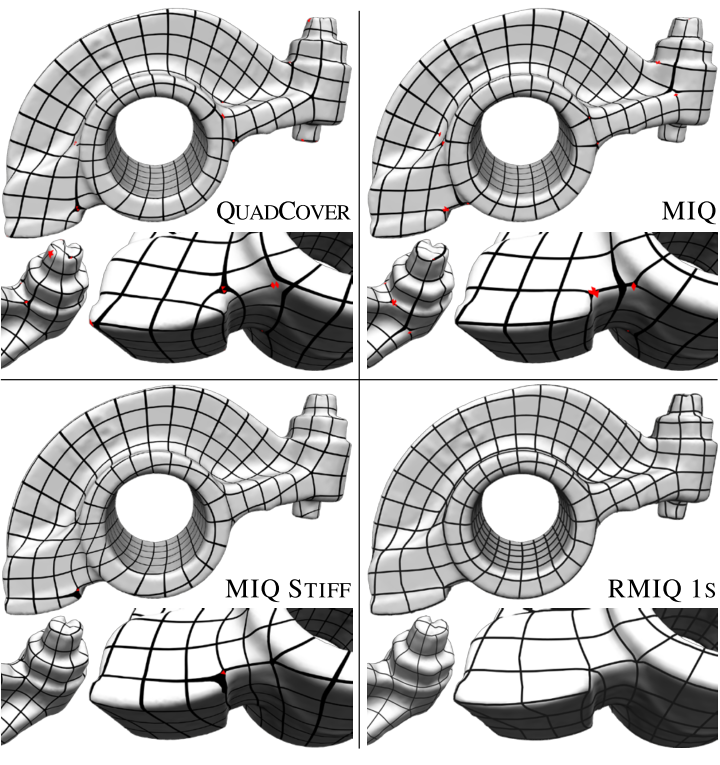
\includegraphics[height=2.5in]{./img/result1.png}
\end{figure}
\end{frame}

\begin{frame}{Results}
\begin{figure}
\centering
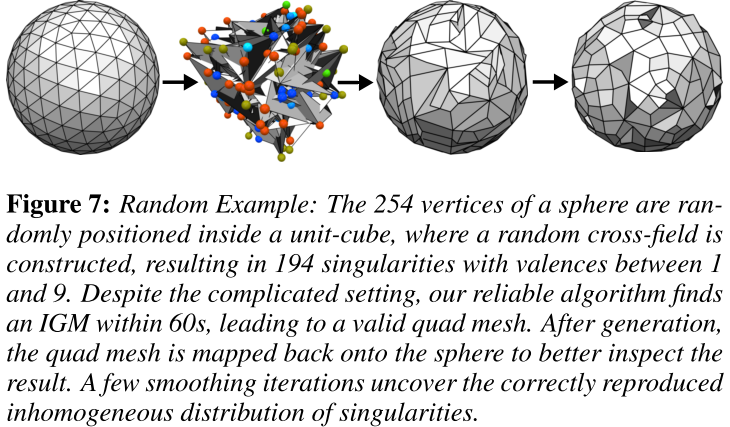
\includegraphics[height=2.5in]{./img/result2.png}
\end{figure}
\end{frame}

\begin{frame}{Results}
\begin{figure}
\centering
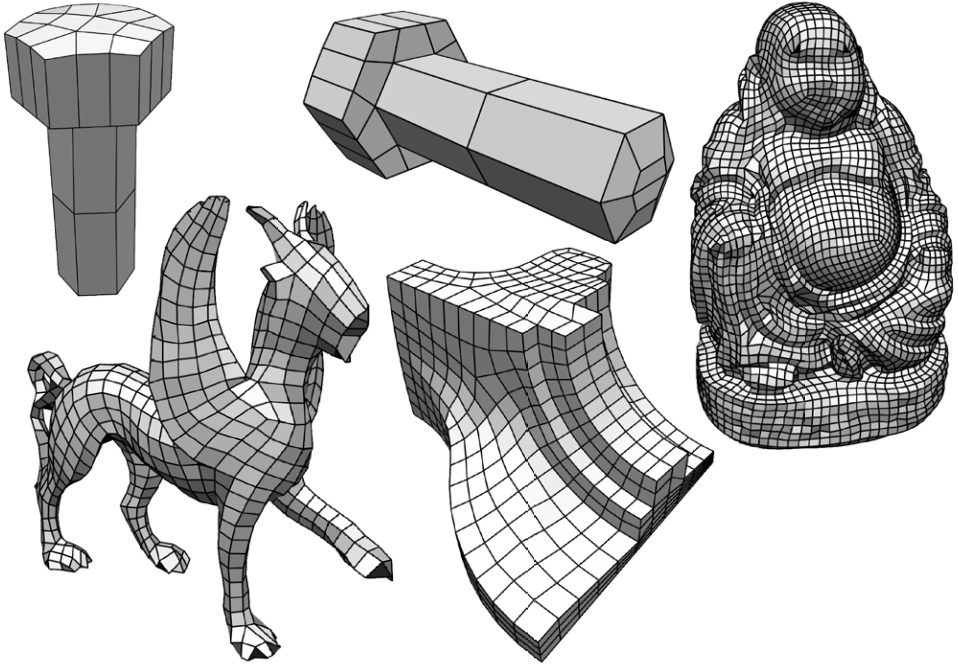
\includegraphics[height=2.5in]{./img/result3.png}
\end{figure}
\end{frame}

\begin{frame}{Results}
\begin{figure}
\centering
\includegraphics[height=2.5in]{./img/result4.png}
\end{figure}
\end{frame}


\section{Conclusion}
\begin{frame}{Conclusion}
\begin{block}{Advantages}
\begin{itemize}
\item Simple idea, good results.
\item Fast convergency.
\end{itemize}
\end{block}
\begin{block}{Drawbacks}
\begin{itemize}
\item This method requires that input metric is smooth, but does not provide a method to design such a metric.
\item Hard to extend it to 3d anistropoic meshing.
\end{itemize}
\end{block}
\end{frame}

\begin{frame}{}
\hspace{1.5in}\huge{Thank you!}
\end{frame}
\end{document}
